%%%%%%%%%%%%%%%%%%%%%%%%%%%%%%%%%%%%%%%%%%%%%%%%%%%
%%%%%%%% Präambel
%%%%%%%%%%%%%%%%%%%%%%%%%%%%%%%%%%%%%%%%%%%%%%%%%%%
\documentclass[a4paper, bibliography=totocnumbered, listof=totocnumbered, oneside, 12pt, ngerman]{scrbook}
\usepackage{geometry}
\geometry{a4paper,left=35mm,right=35mm,top=12mm,bottom=20mm, includeheadfoot}
\setlength\headheight{8mm}

% color
\usepackage{xcolor}
\definecolor{blue}{RGB}{0,128,255}
\definecolor{green}{RGB}{0,128,0}
\definecolor{orange}{RGB}{255,128,0}
\definecolor{lila}{RGB}{128,0,255}
\definecolor{black}{RGB}{0,0,0}

% Absätze
\parindent=0cm

%%%%%%%%%%%%%%%%%%%%%%%%%%%%%%%%%%%%%%%%%%%%%%%%%%%
%%%%%%%% packages
%%%%%%%%%%%%%%%%%%%%%%%%%%%%%%%%%%%%%%%%%%%%%%%%%%%

% speech
\usepackage[utf8]{inputenc}
\usepackage[ngerman]{babel}

% font
\usepackage{lmodern}
\renewcommand\textbullet{\ensuremath{\bullet}}

% hyperlinks
\usepackage[hyphens]{url}
\usepackage[hidelinks]{hyperref}

% math
\usepackage{mathrsfs}

% Bibliothek
\usepackage{bibgerm}
\bibliographystyle{apalike}

% graphics
\usepackage{graphicx}
\DeclareGraphicsExtensions{.pdf,.jpeg,.png,.jpg}

% pseudocode
\usepackage{algpseudocode}

% theorem
\usepackage{amsthm}
\newtheorem{theorem}{Theorem}
\newtheorem{definition}{Definition}

% Codebeispiel
\usepackage{scrhack}
\usepackage{listings}
\renewcommand{\lstlistlistingname}{Quellcodeverzeichnis}
\renewcommand{\lstlistingname}{Codebeispiel}
\lstset{
  backgroundcolor=\color{white},
  basicstyle=\footnotesize,
  breakatwhitespace=false,
  breaklines=true,
  captionpos=b,
  commentstyle=\color{green},
  frame=single,
  keepspaces=true,
  keywordstyle=\color{blue},
  numbers=left,
  numbersep=5pt,
  showspaces=false,
  tabsize=2,
  xleftmargin=0.1\textwidth,
  xrightmargin=0.1\textwidth
}

%%%%%%%%%%%%%%%%%%%%%%%%%%%%%%%%%%%%%%%%%%%%%%%%%%%
%%%%%%%% Document
%%%%%%%%%%%%%%%%%%%%%%%%%%%%%%%%%%%%%%%%%%%%%%%%%%%
\begin{document}
\pagenumbering{roman}

\begin{titlepage}
\begin{centering}
\vspace*{\fill}

\vspace{3cm} 

\textbf { \LARGE
Hypertext-Systeme 1
\\(Lokale Systeme)
\\[1.2cm]
}

{\large
vorgelegt von:
}

\textbf { \Large
Kevin Haack\\[1cm]
}

{\large
Matrikelnummer: 7094226
\\[2mm]
}

{\large
Studiengang: Informatik (M.Sc.)\\[1cm]
}
    
{\large
Thema betreut von:
}

\textbf { \Large
Dr. Felix Winkelnkemper
\\[1cm]
}

{\large
Paderborn, \today
}
\vfill
\end{centering}
\end{titlepage}
\chapter*{Kurzzusammenfassung}

\begin{centering}
\textbf { \LARGE
Security of Symmetric Encryption against Mass Surveillance
\\[1.2cm]
}
\end{centering}

{\large
Zusammenfassung
}

{
Spätestens seit den Snowden Leaks ist öffentlich bekannt, dass Massen"-über"-wachung im Internet stattfindet. Codenamen wie PRISM werden in Zeitschriften ver"-öffentlicht (\cite{Guard}). Wir sehen, dass verschlüsselte Übertragungen unsere Daten nicht vor unbefugtem Zugriff schützen. Pseudozufallsgeneratoren die möglicherweise nicht ganz zufällig sind, wie zum Beispiel der NIST Dual EC DRBG, sorgen für potenziell unsichere VPN Verbindungen und Backdoors in eigentlich sicheren Übertragungen (\cite{dual}) könnten in nahezu jeder Anwendung vorkommen. Das original Paper von Mihir Bellare, Kenneth G. Paterson und Phillip Rogaway soll die erste Salve im Kampf gegen Massenüberwachung abgeben (\cite{praesi}) und fokussiert sich auf symmetrische Verschlüsselungsschemen und einen speziellen Angriffsvektor, den sogenannte Algorithm Substitution Attacks. Es soll eine Grundlage mit der Definition und Formalisierung schaffen für die Abwehr dieses Angriffs. Denn symmetrische Verschlüsselungen bilden das Rückkrad vieler alltäglicher Übertragungs"-techniken wie zum Beispiel IPsec oder TLS. Diese Arbeit soll zunächst einen Überblick über das Originalwerk geben, Inhalte zusammenfassen und verdeutlichen. Es wird dargestellt, wie Algorithm Substitution Attacks funktionieren könnten und welchen symmetrische Schemen dagegen gefeit sind.
}\vspace{12pt}

{\large
Stichworte
}

{
Algorithm Substitution Attacks, symmetrische Verschlüsselung, unique ciphertext scheme, key recovery
}

\tableofcontents
\cleardoublepage
\pagenumbering{arabic}

\chapter{Was ist Hypertext?}
\label{ch:Was ist Hypertext?}

\begin{section}{Was ist überhaupt Hypertext?}
\label{sec:big_brother}

Was ist überhaupt Hypertext? Nach Jakob Nielsen in dem Buch Multimedia and Hpertext: The Internet and Beyond aus dem Jahr 1995, ist:

\begin{quote}
\glqq The simplest way to define hypertext is to contrast it with traditional text like a book. All traditional text, whether in printed form or in computer files, is sequential, meaning that there is a single linear sequence defining the order in which the text is to be read. [...] Hypertext is nonsequential; there is no single order that determines the sequence in which the text is to be read.\grqq{ }\cite[S.1]{Nielsen1995}
\end{quote}

Jakob Nielsen beschreibt, genau wie Jeff Conklin in seinem Artikel Hypertext: An Introduction and Survey, Hypertext als Informationsquelle die dem Leser die Freiheit gibt die Informationen in beliebiger Reihenfolge abzurufen. Der Leser dürfe entscheiden, welche Links er nutze und in welcher Reihenfolge \cite[S.33]{Conklin1987} \cite[S.1]{Nielsen1995}.

\begin{quote}
\glqq Hypertext allows and even encourages the writer to make such references, and allows the readers to make their own decisions about which links to follow and in what order. In this sense, hypertext eases the restrictions on the thinker and writer. It does not force a strict decision about whether any given idea is either within the flow of a paper's stream of thought or outside of it.\grqq{ }\cite[S.33]{Conklin1987}
\end{quote}

Also könnte ein Hypertext wie auf Abbildung \ref{fig:nielsenLink} zu sehen, aus vielen einzelnen Informationen bestehen zwischen denen eine Verlinkung existiert. Durch diese Links kann der Leser entscheiden an welcher Stelle er weiter lesen möchte. Anstatt den Text in der festen Reihenfolge $A$, $B$, $C$, $...$ und dann $G$ zu lesen, gibt es für den Leser mehrere Möglichkeiten die Texte aufzurufen. Nach Text $A$ könne zum Beispiel sofort Text $D$ folgen und so weiter\cite[S.1]{Nielsen1995}.

\begin{figure}[H]
	\centering
	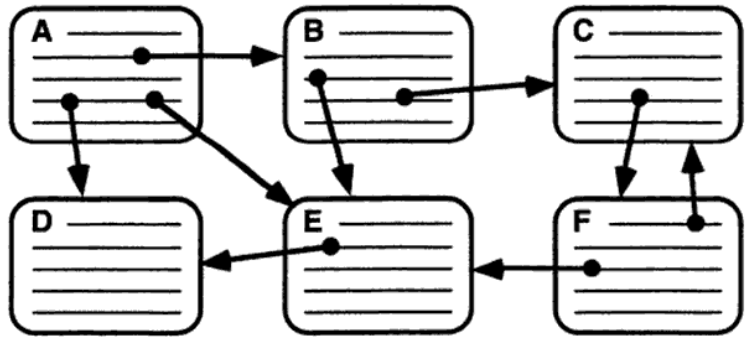
\includegraphics[width=0.8\textwidth]{image/nielsenLink}
	\caption{Vereinfachte Ansicht eines Hypertextes \cite[S.1]{Nielsen1995}}
	\label{fig:nielsenLink}
\end{figure}


Einen Hypertext kann oftmals als Graphen aus Knoten und Kanten dargestellt werden. Diese Darstellungsform kann vor dem Leser verborgen sein, muss es aber nicht \cite{Conklin1987}. Eine Information, ein Absatz, ein Text oder ein Dokument ist ein Knoten, die Größe spielt hierbei keine Rolle. Ein Knoten kann nun Links auf andere Knoten haben und diese sind dann die Kanten in dem Graphen \cite[S.19]{Conklin1987} \cite[S.2]{Nielsen1995}. Auch John B. Smith und Stephen F. Weiss schreiben in dem Artikel Hypertext vergleichbar über Hypertext als Netzwerk aus Informationen mit Links \cite{Smith1988}. Diese bezeichnen unter anderem auch Verlinkungen zwischen Medien wie Audio-, Grafik- oder Videodateien als Hypertext. In diesem Zusammenhang verwendet Theodor \glqq Ted\grqq{ }Holm Nelson auch den Begriff \glqq Hypermedia\grqq{ }\cite{Nelson1965}.

\begin{quote}
    \glqq [...] Hypertext is an approach to information management in which data is stored in a network of nodes connected by links. Nodes can contain text, graphics, audio, video, as well as source code or other forms of data.\grqq{ }\cite{Smith1988}
\end{quote}

Wie auf Abbildung \ref{fig:imText} zu sehen, müsse eine Link also nicht unbedingt von Wort zu Wort führen, sondern könne auch den Token $xxxx$ im Dokument $A$ mit dem ganzen Dokument $B$ verbinden \cite{Conklin1987}. 

\begin{figure}[H]
	\centering
	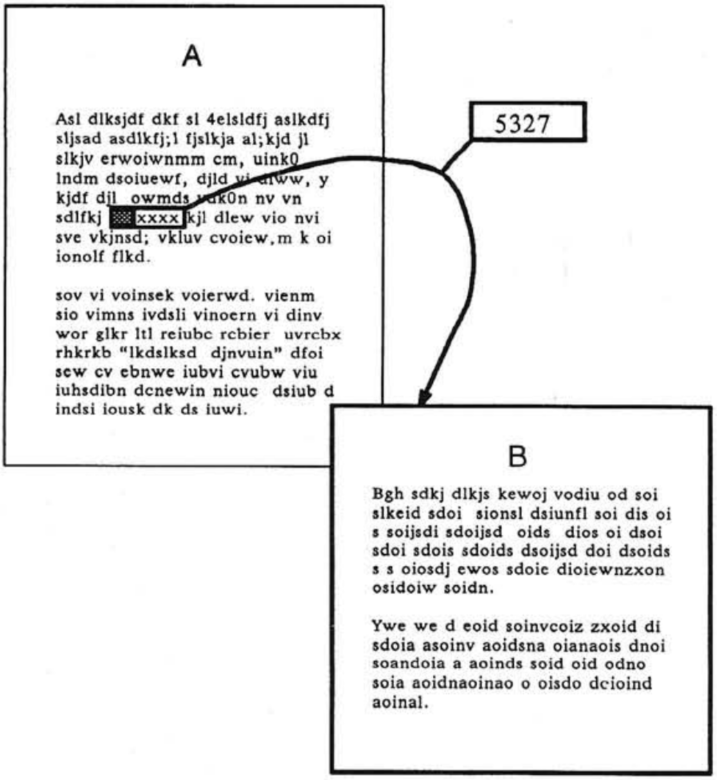
\includegraphics[width=0.8\textwidth]{image/imText}
	\caption{Ein Beispiel eines Links von in einem Text zu einem anderen Text \cite[S.34]{Conklin1987}}
	\label{fig:imText}
\end{figure}

\begin{quote}
    \glqq The same is true of footnotes in traditional printed texts, since readers have to determine upon reaching the footnote marker whether to continue reading the primary stream of text or to branch off to pursue the footnote. \grqq{ }\cite{Nielsen1995}
\end{quote}

Das gleiche könne auch auf einen traditionellen Text auf Papier zutreffen, Fußnoten referenzieren auf andere Texte und geben dem Leser die Möglichkeit an anderer Stelle weiterzulesen \cite{Nielsen1995}. Auch Ted Nelson schrieb in Literary Machines 1992:

\begin{quote}
\glqq By hypertext I simply mean non-sequential writing. A magazine layout, with sequential text and insert illustrations and boxes, is thus hypertext.\grqq{ }\cite{Nelson1992}
\end{quote} 

\end{section}

\begin{section}{Abgrenzung}
\label{sec:abgrenzung}

Doch für eine Antwort auf die Frage was ein Hypertext ist, gibt es sicherlich noch viele andere Antworten und Definitionen. Doch im Jahr 1945 veröffentlichte Vannevar Bush den Artikel \glqq As we may think\grqq{ }und formulierte darin die Grundidee zu Hypertext. Ich beschränke mich in dieser Arbeit auf lokale Hypertext-Systeme insbesondere der achtziger Jahre. Ich nehme in dieser Arbeit Bezug auf ausgewählte Hypertext-Systeme, deren Benutzung, Funktionen und technische Umsetzung. Ein besonderes Augenmerk legt diese Arbeit hierbei auf die Umsetzung der Links. Vernetzte und verteilte Hypertext-Systeme klammere ich in dieser Arbeit explizit aus.

\end{section}

\chapter{Geschichtliches}
\label{ch:Geschichtlich}

In der Geschichte von Hypertext bis Heute sind viele verschiedene Konzepte und Systeme entstanden. In diesem Kapitel werden für einen Überblick einige davon vorgestellt. Das Konzept hinter Hypertext kann auf einen Artikel aus dem Jahr 1945 zurückgeführt werden.

\begin{quote}
	\glqq Consider a future device for individual use, which is a sort of mechanized private file and library. It needs a name, and to coin one at random, memex will do. A memex is a device in which an individual stores all his books, records, and communications, and which is mechanized so that it may be consulted with exceeding speed and flexibility.\grqq{ }\cite[Section 6]{Bush1945}.
\end{quote}

Im Jahr 1945 wurde \glqq As we may think\grqq{ }von Vannevar Bush veröffentlicht. Mit dem Konzept \glqq Memex\grqq{ } erdachte Vannevar Bush eine Maschine für die individuellen Verwendung - eine private, mechanisierte Bibliothek. Die Abbildung \ref{fig:memex} zeigt eine Illustration aus dem Life Magazine 1945. Wenn der Nutzer ein bestimmtes Buch aufrufen möchte, könne er einen Code in das Keyboard eintippen und die Titelseite erscheint als Projektion \cite[S.121]{Life1945} \cite[Section 6]{Bush1945}. 

\begin{figure}[H]
	\centering
	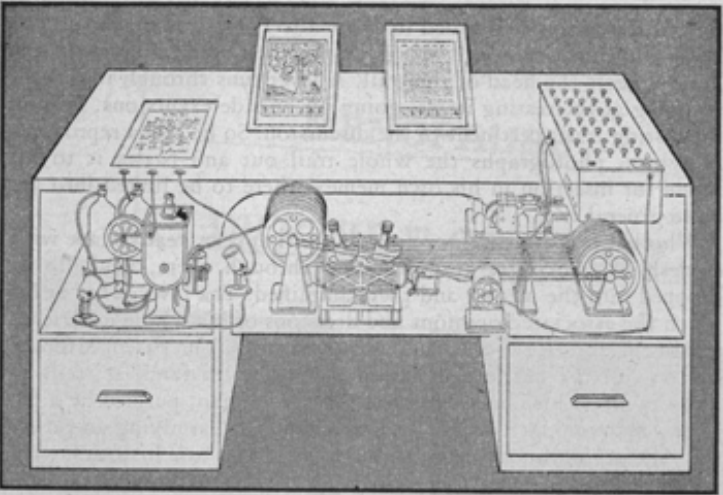
\includegraphics[width=0.7\textwidth]{image/memex}
	\caption{\glqq Memex in the form of a desk would instantly bring files and material on any subject to the operator's fingertips. [...] At left is a mechanism which automatically photographs longhead notes, pictures and letters, then files them in the desk for future reference\grqq{ } \cite[S.123]{Life1945}}
	\label{fig:memex}
\end{figure}

In in diesem Konzept solle der Nutzer einen sogenannten \glqq main trail\grqq{ }aus Dokumenten erstellen. Dieser Trail sei eine Kombination aus Dokumenten, die aus der Perspektive des Nutzers von Interesse ist. Mit sogenannten \glqq side tails\grqq{ }sollte der Nutzer ein Main Trail mit anderen Dokumenten \glqq assoziieren\grqq{ }\cite[Section 7]{Bush1945}. Diese Side Trails könnten als erstes Konzept von Hyperlinks verstanden werden. Zwei Jahrzehnte nach der Veröffentlichung von \glqq As we may think\grqq{ }, in der 1960er Jahren, wurde erst der Begriff Hypertext von Theodor \glqq Ted\grqq{ }Holm Nelson geprägt. 

\begin{quote}
	\glqq Let me introduce the word hypertext to mean a body of written or pictorial material interconnected in such a complex way that it could not conveniently be presented or represented on paper. It may contain summaries, or maps of its contents and theier interrelations; it may contain annotations, additions and footnotes from scholars who have examined it. [...]\grqq{ }\cite{Nelson1965}
\end{quote}

Nach Ted Nelson habe ein System auf Papier gravierende Einschränkungen beim Organisieren oder Präsentieren von Ideen. Ein Buch könne nie perfekt zu einem Leser passen. Der eine Leser sei gelangweilt, während ein anderer von den gleichen Seiten verwirrt werde. \glqq Ein solches System könne das Potenzial haben, das Gefühl der Freiheit, die Motivation und das intellektuelle Verständnis des Lesenden zu vergrößern\grqq{ }\cite{Nelson1965}. 

\begin{section}{NLS und AUGMENT}
\label{sec:nls}

Im gleichen Jahrzehnt erschien Doug Engelbarts \glqq Augmenting Human Intellect: A Conceptual Framework\grqq{ }. Er schrieb unter anderen von dem \glqq digital computer as a tool for the personal use of an individual. Here there is not only promise of great flexibility in the composing and rearranging of text [...]\grqq{ }\cite[S. 17]{Engelbart1962}.

\begin{quote}
\glqq By augmenting human intellect we mean increasing the capability of a man to approach a complex problem situation [...].\grqq{ }\cite[S. 1]{Engelbart1962}
\end{quote}

Während seiner Arbeit am Augmentation Research Center am Stanford Research Institute (SRI-ARC) wurde unter anderem das \glqq NLS\grqq{ }(the oN-Line System) entwickelt. Wobei \glqq on-line\grqq{ }in den 60er Jahren nicht die gleiche Bedeutung gehabt haben dürfte als Heute. Vorgestellt wurde das NLS auf der Fall Joint Computer Conference in San Francisco 1968. Diese Präsentation wird oft \glqq mother of all demos\grqq{ }genannt. Neben dem NLS wurden auch die interaktive Textverarbeitung, die Computermaus und die Organisation von Windows auf dem Bildschirm vorgestellt (Siehe Abbildung \ref{fig:mother}). Das NLS wurde präsentiert als \glqq ein mächtiges Tool für die Arbeit eines Individuums, wenn er studiert, plant, designt, debuggt oder dokumentieren.\grqq{ }\cite{MotherOfDemo1968}. Es gab Möglichkeiten für das kollaborative Arbeiten, gemeinsame Dokumente und man konnte Nachrichten an Dokumente heften \cite{MotherOfDemo1968}. 

\begin{figure}[!ht]
	\centering
	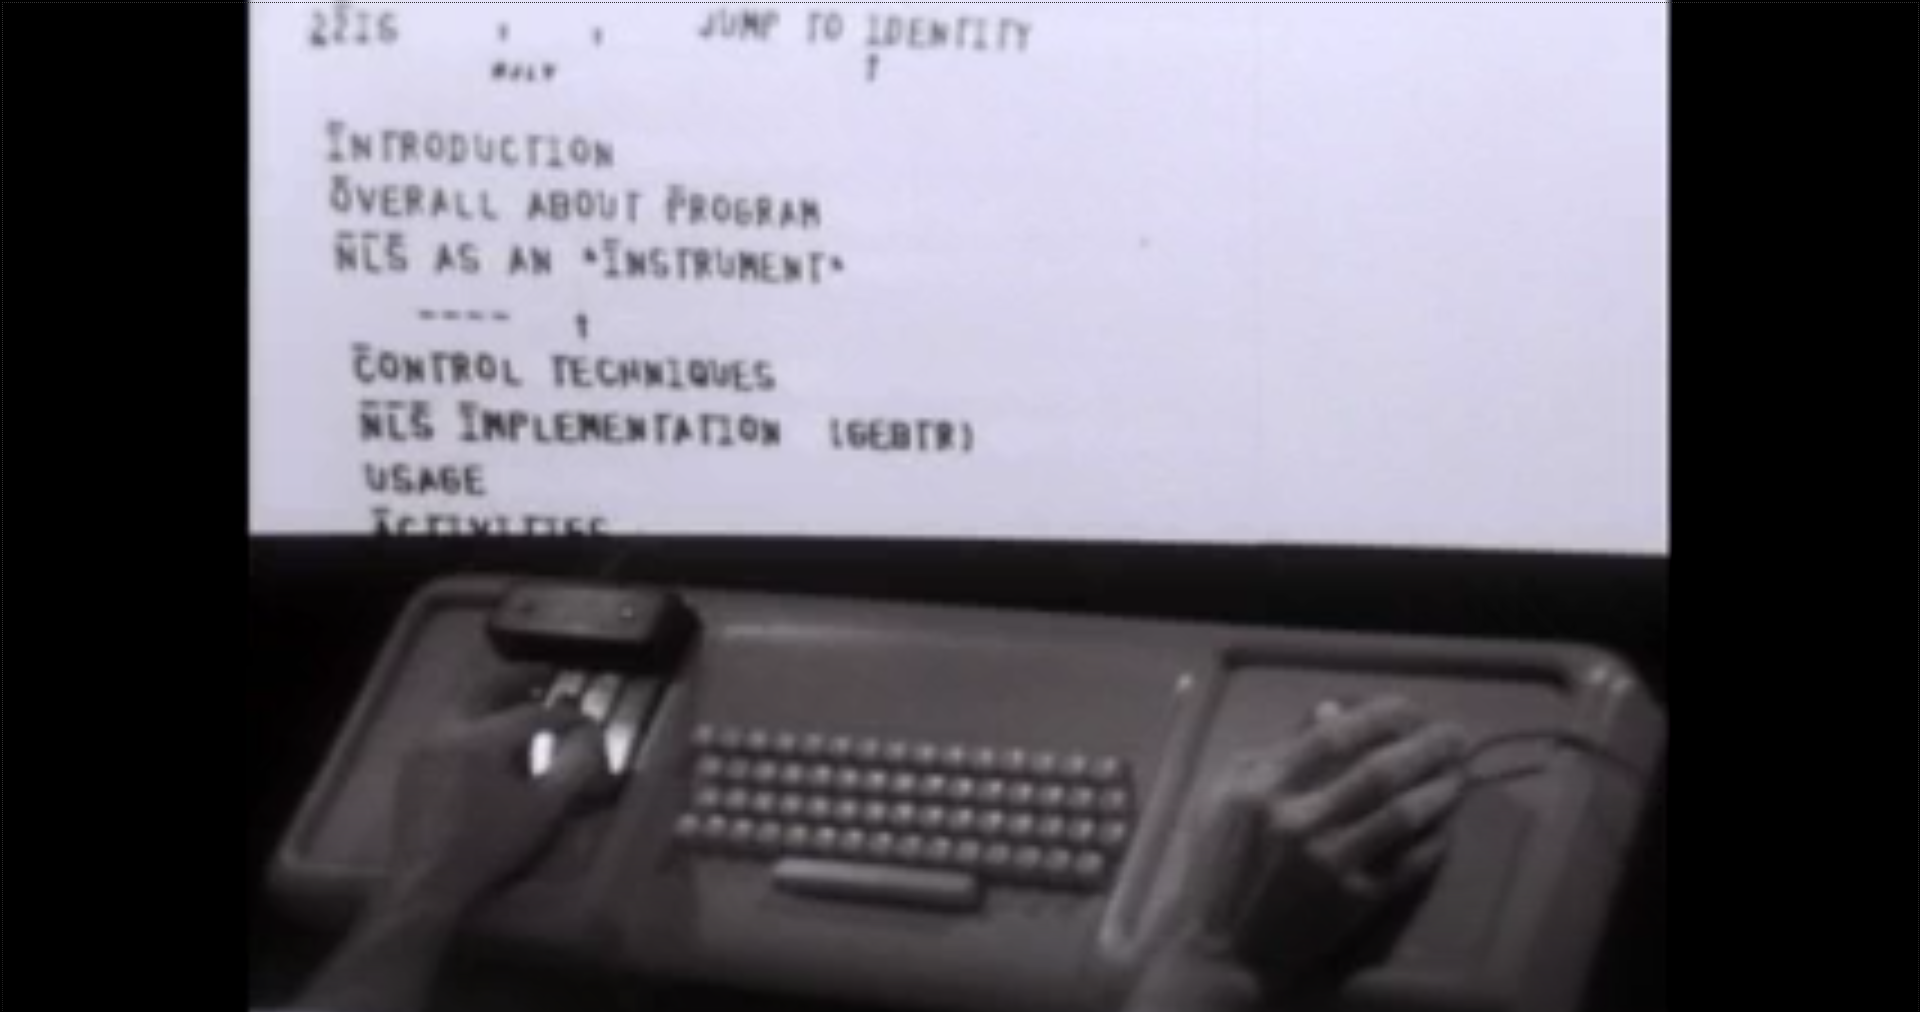
\includegraphics[width=0.9\textwidth]{image/mother}
	\caption{Doug Engelbart präsentiert auf der Fall Joint Computer Conference in San Francisco die Forschung vom Stanford Research Institute \cite{MotherOfDemo1968}.}
	\label{fig:mother}
\end{figure}

Gezeigt wurden aber auch die Hypertext Funktionalitäten, Dokumente seien verknüpft mit Links und der Nutzer könne entscheiden welchen \glqq Branch\grqq{ }er betrete \cite{MotherOfDemo1968}. Verlinkungen konnten durch verschiedene Adressiermöglichkeiten realisiert werden. Jedes Dokument in NLS ist in \glqq Statements\grqq{ }unterteilt und diese Statements konnten auf verschiedene Weisen verlinkt werden. Um ein Statement eindeutig zu identifizieren, wurden dem Nutzer vier Möglichkeiten zur Verfügung gestellt \cite{Engelbart1984}: 

\begin{itemize}
\item Structural Statement Number\hfill \\
Die \glqq Structural Statement Number\grqq{ }bezeichnet die strukturelle Position des Statements. Das System vergibt diese Nummber anhand der Position innerhalb eines Dokumentes. Diese Nummern konnten zum Beispiel dargestellt werden als $1$, $1a$, $1a1$ und $1b$. Durch das Verändern der Dokumentenstruktur wurden vom System allerdings neue Nummern vergeben, so konnten Verweise auf falsche oder nicht mehr existierende Statements zeigen.
\item Statement Identifier (oder SID)\hfill \\
Der \glqq Statement Identifiers\grqq{ }, als globale ID war unabhängig von der Position des Statements, diese Nummer wurde sequenziell vom System vergeben und wurde nie verändert. Diese Nummern wurden immer mit der \glqq 0\grqq{ }als Präfix angezeigt.
\item Worker-Assigned Statement Name (oder label)\hfill \\
Die \glqq Labels\grqq{ }konnten vom Nutzer definiert werden. Der Nutzer konnte Trennzeichen angeben, mit denen das System dem Statement einen Namen gibt. Wenn zum Beispiel die Trennzeichen \glqq (\grqq{ } und \glqq )\grqq{ }gewählt wurden, erkannte das System das erste eingeklammerte Wort als Label.
\item Direct Screen Selection\hfill \\
Die letzte Möglichkeit war die \glqq Direct Screen Selection\grqq, der Nutzer konnte mit der Maus den Cursor auf ein Statement bewegen und mit dem Drücken von \glqq Select\grqq{ } auf der Maus das entsprechende Statement auswählen. Diese letzte Möglichkeit diente zur Textmanipulation.
\end{itemize}

Das Userinterface bot Kommandos zum Manipulieren der Oberfläche. Die interaktive Textbearbeitung unterstützte Funktionen wie Insert, delete, Move and Copy. Es konnten Outlines und eine Vorschau der ersten Zeilen von jedem Statement angezeigt werden. Die Verlinkungen und Bedienmöglichkeiten ermöglichten dem Nutzer ein \glqq herein und heraus zoomen \grqq{ }\cite{MotherOfDemo1968}. Die kommerziellen Rechte an dem System wurden 1978 an Tymshare abgegeben und NLS wurde zu AUGMENT umbenannt \cite{Engelbart1984}. Im Vergleich zum Konzept Memex hatte das Team um das NLS ähnliche Ziele, denn in beiden Projekten sollte die die Arbeit des Individuums optimiert werden \cite{Life1945} \cite{MotherOfDemo1968}. Die Verknüpfungen der Dokumente in der Memex sind vergleichbar mit den verlinkten Statements im NLS, beide Verlinkungen wurden über IDs realisiert \cite{Engelbart1984}, \cite{Bush1945}, nur die Navigation durch die Links unterschied sich bei beiden, statt berührungssensitive Anzeige und Spracheingabe \cite{Bush1945}, nutzte das Team rund um Doug Engelbart Maus und Tastatur \cite{MotherOfDemo1968}.

\end{section}

\begin{section}{Problem: Dangling edges}
\label{sec:dangling}

Allerdings wäre Vannevar Bush bei einer Realisierung der Memex wahrscheinlich auf das gleiche Problem gestoßen wie Doug Engelbart. Ein Hypertext ist vergleichbar mit einem Graphen aus Knoten und Kanten. Ein Text ist ein Knoten und die Verlinkungen zwischen den Texten sind die Kanten zwischen den Knoten. Durch entfernen von Knoten können sogenannte \glqq dangling edges\grqq{ }entstehen, eine Kante, die ein Start hat aber kein Ziel mehr. Die Abbildung \ref{fig:dangle} zeigt zum Beispiel durch das Entfernen des Textes $D$ zwei entstandenen Dangling Edges von $A$ und $E$. Bei NLS konnte durch das Bearbeiten der Dokumente oder Statements Dangling Edges entstehen. Dies könnte durch die verschiedenen Adressiermöglichkeiten zumindest eingedämmt werden \cite{Engelbart1984}.

\begin{figure}[H]
	\centering
	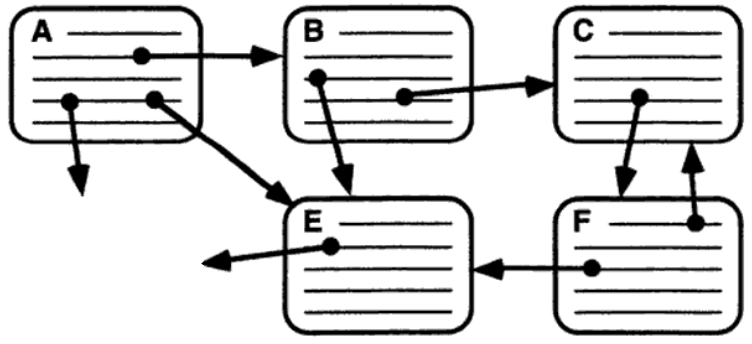
\includegraphics[width=0.9\textwidth]{image/dangle}
	\caption{Modifizierte Darstellung von Nielsen, zur Darstellung von zweier Dangling Edges \cite[S.1]{Nielsen1995}.}
	\label{fig:dangle}
\end{figure}

\end{section}

\begin{section}{HES}
\label{sec:hes}

Ebenfalls in dem 1960er Jahren wurde an der Brown Universität, im US-amerikanischen Bundesstaat Rhode Island, ein Hypertext-System Namens \glqq HES\grqq{ } (Hypertext Editing System) entwickelt. 1967 begannen Andries van Dam und Ted Nelson die Entwicklung an HES. Eigentlich sei der Zweck von HES gewesen, das Hypertext Konzept zu erforschen, später sei es von IBM aber auch an die NASA verkauft worden und zur Dokumentation der Apollo Missionen verwendet worden \cite{Dam1988}.

\begin{quote}
\glqq One of the most important things (Nelson) taught me was that this is a new medium and you really can’t be constrained to thinking about it in the old ways. Don‘t copy old, bad habits; think about new organizations, new ways of doing things, and take advantage of this new medium.\grqq{ }\cite{Dam1988}
\end{quote}

Texte konnten in HES in separate Sektionen unterteilt werden. Grundlegend gab es zwei verschiedene Verlinkungen in HES, \glqq Links\grqq{ }und \glqq Brachnes\grqq{ }. Branches wurden organisiert im Branch Menü oder waren im späteren Ausdruck als Fußnoten zu sehen. Links konnten optional vom Nutzer besucht werden. Beide waren im Text markiert mit einem Sternchen (*) und zeigten einen sogenannten Explainer als Vorschau an. Der Explainer eines Links tauchte in der Annotaion Area auf, der Branch Explainer wurde in-line beim Branch Sternchen angezeigt. Der Nutzer konnte Sektionen mit dem Lightpen auswählen und einem einzigartigem Label versehen. Dieses Label wurde dann in eine Label Tabelle eingetragen werden und konnten mit dem Befehl besucht werden und als Pointer in einem Text verwendet werden \cite{Dam1969}. Die Texte selbst waren sogenannte Instanzen und wurden unidirektional verlinkt. Die Bearbeitung selbst sei mehr eine Pointer Manipulation als Text Manipulation gewesen \cite[S. 890]{Dam1988}.

\begin{figure}[H]
	\centering
	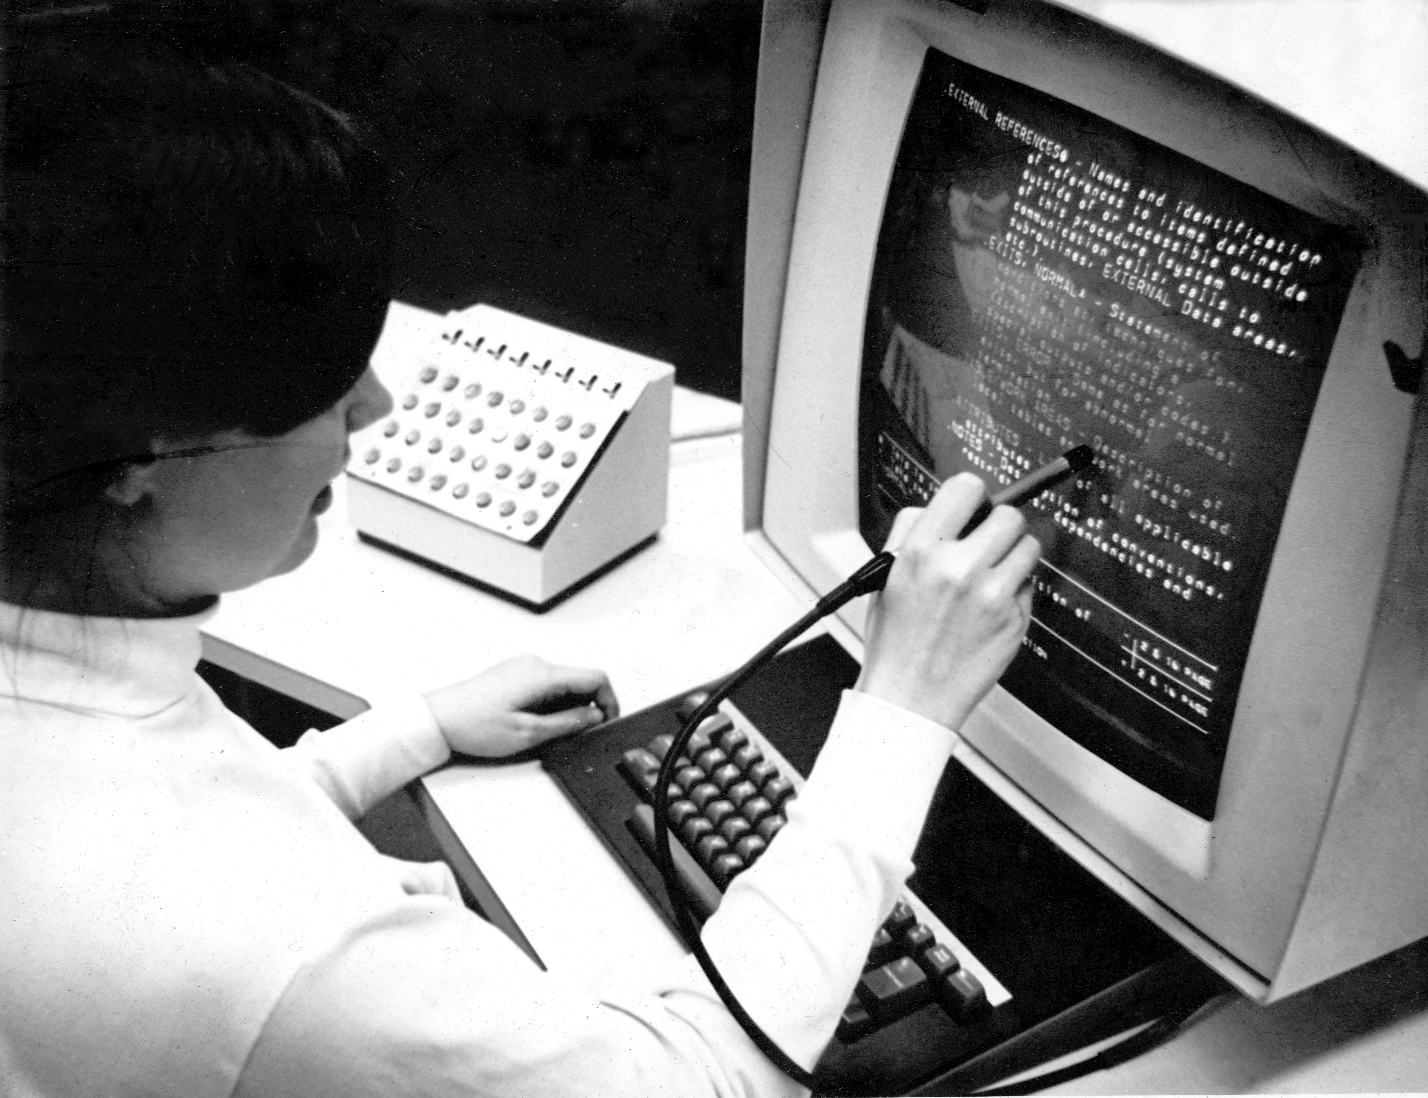
\includegraphics[width=0.8\textwidth]{image/hes}
	\caption{Foto einer von HES in der Brown Universität \cite{Lloyd1969}.}
	\label{fig:hes}
\end{figure}

\begin{quote}
\glqq Instances are references, so that if you changed, for example, a piece of legal boilerplate that was referenced in multiple places, the change would show up in all the places that referenced it. \grqq{ }\cite{Dam1988}
\end{quote}

Dem Nutzer war die Möglichkeit gegeben, nach dem Drücken eines \glqq Function Keys\grqq{ }mit dem Lightpen einen Link zu berühren und so dem Link zu folgen \cite[S.23]{Dam1969}. Wie auch das NLS unterstützte die Textbearbeitung Funktionen wie Insert, Delete, Move and Copy \cite[S.10-14]{Dam1969}, \cite[S. 889]{Dam1988}. Beim entfernen vom Texten entstanden keine Dangling Edges, wie in Abschnitt \ref{sec:dangling} beschrieben. Da jeder Link oder Branch, der auf die gelöschte Sektion zeigte, ebenfalls gelöscht wurde \cite[S.12]{Dam1969}.

\end{section}

\begin{section}{FRESS}
\label{sec:fress}
	
1968 startete van Dam zusammen mit seinen Stunden die Entwicklung von \glqq a File Retrieval and Editing System\grqq{ }(FRESS). Inspiriert von Doug Engelbart sollte FRESS die besten Ideen von NLS und HES vereinen \cite[S.887 und 890]{Dam1988}. Im Gegensatz zu vorherigen Systemen solle FRESS auch auf verbreiteten kommerziellen Systemen laufen. Van Dam zufolge sei FRESS das erste System gewesen, dass eine UNDO Funktion unterstützte. Jede Bearbeitung wurde in einener Schattenversion gespeichert und erlaubte so ein Autosave und ein UNDO \cite[S.891]{Dam1988}.

\begin{figure}[H]
	\centering
	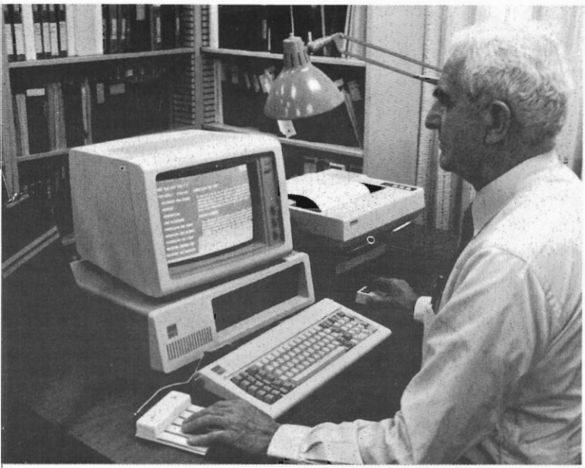
\includegraphics[width=0.9\textwidth]{image/augment}
	\caption{Engelbart an einer NLS/Augment Workstation. Das Key Set unter seiner linken Hand und die Maus unter seiner rechten Hand. \cite{Conklin1987}.}
	\label{fig:augment}
\end{figure}

Im Gegensatz zum Vorgänger unterstützte FRESS bidirektionale Links, so genannte \glqq Jumps\grqq{ }. Aber weiterhin gab es auch on-way Links, die sogenannten \glqq Tags\grqq{ }. Paul Delany und George P. Landow schrieben hierzu: 

\begin{quote}
\glqq FRESS had two types of links - indicated a connection to a single element such as an annotation, definition, or footnote. When the reader pointed to a tag with a light pen, the associated text appeared in another window on the screen for reference while the reader remained in the main document. Unlinke a tag, a jump - a bidirectional link - indicated a path to another document. By following a jump, the reader was transferred from one document to another, and up to seven windows could be used to display documents simultaneously. \grqq{ }\cite[S.68]{GeorgeLandow1995}
\end{quote}

FRESS unterstütze so den Nutzer beim Navigieren durch die Links, außerdem konnte so der Autor, wie schon bei der Memex angedacht, eine Art Main Track oder Side Tracks erstellen. Im Dokument wurden die \glqq cross-reference markers\grqq{ }angezeigt, diese zeigten dem Nutzer alle Verlinkungen an und gaben dem Leser einen \glqq Backtrack\grqq{ }durch seine besuchten Links. Links waren in FRESS eigene Objekte und nicht mehr einfach Teile eines Textes. Es sei möglich gewesen Links zu typisieren oder zu labeln, indem man sie mit \glqq key words\grqq{ }versehe \cite[S.891]{Dam1988}. Das System wurde auf Grund des hohen Funktionsumfang nicht fertig gestellt, van Dam schrieb \glqq It was overkill, and we haven’t done it since, but it certainly was interesting.\grqq{ }\cite[S.891]{Dam1988}.

\end{section}

\begin{section}{Problem: Lost in Hyperspace}
\label{sec:lostInHyperspace}

Je komplexer und größer ein Hypertext Graph wird, desto einfacher kann man sich auf der viel zahl von Branches verlieren. So auch van Dam: \glqq We already started getting the notion that the richer the hypertext, the greater the navigational problem. \grqq{ }. Nach van Dam sei das \glqq come from\grqq{ } genauso wichtig wie das \glqq go to\grqq{ }\cite{Dam1988}.

\begin{quote}
\glqq [...] The real diagram was about the size of a large blueprint [...]. We had already come to the point where Ted, who designed it, was able to go through the hypertext pretty well, but some of the rest of us had difficulty following it-it was not exactly obvious where you were. This, of course, is the classical lost-inhyperspace problem [...]\grqq{ }\cite{Dam1988}
\end{quote}

FRESS nutzte beim Aufruf von Links beispielsweise Windows bidirektionale Links damit der Nutzer jederzeit einen Weg zurück fand. Bei einer Umsetzung der Memex ist zu vermuten, dass dieses Problem durch die zwei Anzeigen zumindest entschärft worden wäre, aber auch hier wäre man beim Navigieren durch die Dokumente irgendwann \glqq lost in hyperspace\grqq gewesen. Erst die bidirektionalen Links und Windows lösen dieses Problem und geben dem Nutzer die Möglichkeit seinen Weg zurück zugehen.

\end{section}

\begin{section}{Document Examiner}
\label{sec:DocumentExaminer}

Die ersten Hypertext-Systeme wie NLS und FRESS haben gezeigt, dass Hypertext nicht nur ein Konzept sind, sondern auch als echte Systeme implementiert werden können. In den achtziger Jahren kamen dann einiger mehr auf. Eines davon war im Jahr 1985, Document Examiner von Symbolics. Document Examiner diente zur Anzeige der Handbücher und der Dokumentation der Symbolics Systeme, war also nicht für akademische oder forschungs Zwecke, sondern kommerzielle Zwecke gedacht \cite{Walker1987}, \cite[S. 50]{Nielsen1995}. Anders als bei den vorherigen System sei es Ziel bei der Entwicklung von  Document Examiner gewesen, die Oberfläche handhabbar wie ein Buch zu gestalten und dabei Vorteile einer nicht-Papier-Lösung hinzuzufügen \cite{Walker1987}. Durch die Buch Metapher solle die Anwendung benutzerfreundlicher als andere Systeme werden \cite{Walker1987}. 

\begin{quote}
\glqq The most fundamental decision in the interface was to make the material that a person was reading look essentially as it would in a paper book. The reason for doing this was "ease of use". We saw no reason to have the underlying information structure be reflected in the user interface model unless that structure was a good model for interacting with information. My experience in trying to help users with a tree-structured information interface [...] led me to believe that a book-like interface would be more palatable for many people. \grqq{ }\cite{Walker1987}
\end{quote}

\begin{figure}[H]
	\centering
	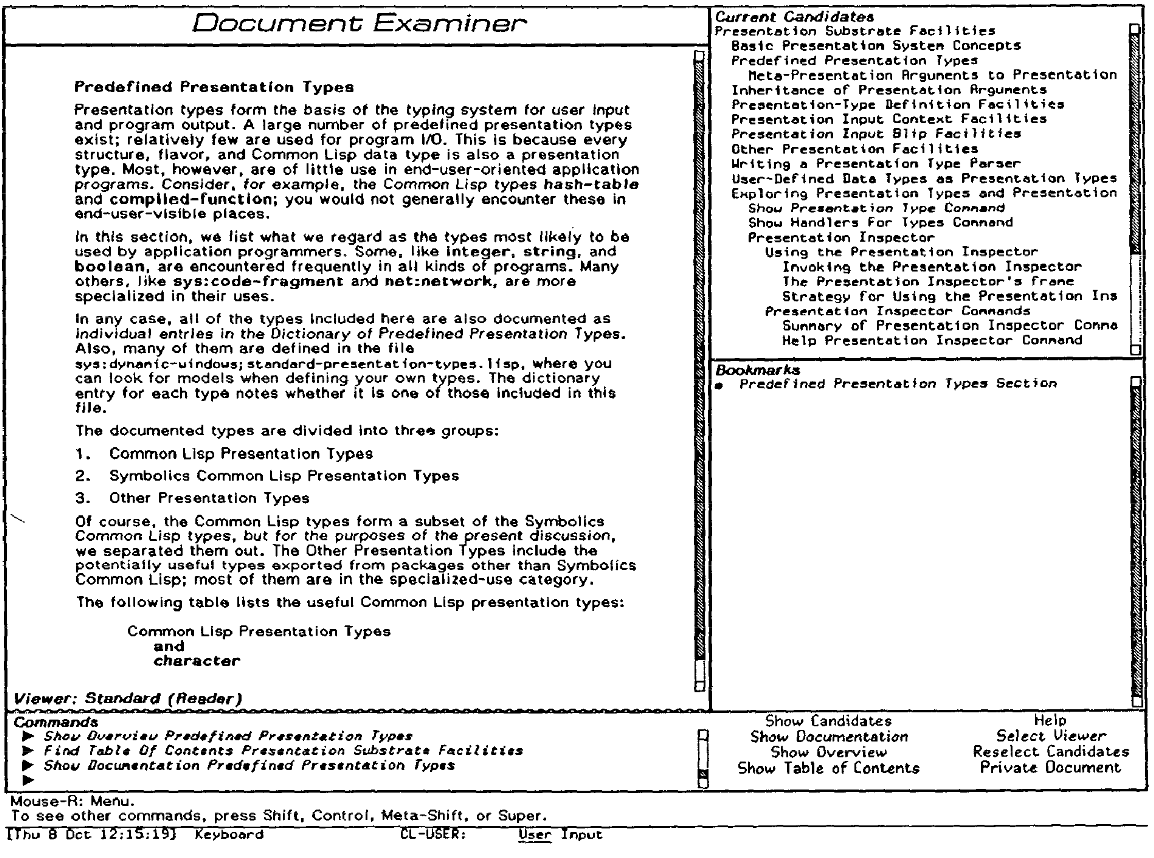
\includegraphics[width=0.8\textwidth]{image/document}
	\caption{Userinterface von Document Examiner. Zeigt die vier Abschnitte: Content Area, Bookmark Pane, Candidates Pane und Command Region \cite{Walker1987}.}
	\label{fig:ducument}
\end{figure}

Document Examiner wurde als \glqq window-based\grqq{ }bezeichnet, wie auf Abbildung \ref{fig:ducument} zusehen, unterteilen die Windows die Anwendung in vier Abschnitte. Die Conent Area, zum Anzeigen des Inhalts. Die Bookmark Pane, enthält eine chronologische Aufzählung der Records, die der Benutzer gelesen hat. Die Command Pane, die dem Nutzer es ermöglicht Befehle abzusetzen \cite{Walker1987}. Die Candidates Pane, enthält die vom Nutzer zusammengestellten Records, die noch zu lesen sind. Die Liste der Candidates war wie ein Suchergebnis, der Nutzer konnte einen Befehl absetzen, mit dem er nach Bestimmten Begriffen im Titel oder in den Keywords suchen konnte. Abbildung \ref{fig:candidates} zeigt eine Suchanfrage und das Ergebnis eines solchen Befehls.

\begin{figure}[H]
	\centering
	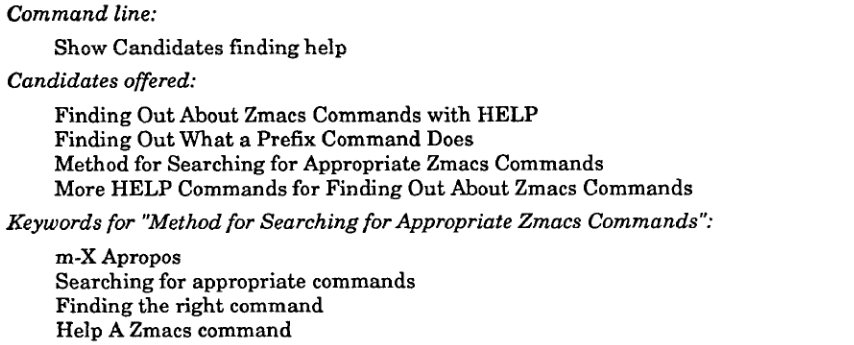
\includegraphics[width=0.9\textwidth]{image/candidates}
	\caption{Zeigt die vorgeschlagenen Records, die mit dem Befehl $show candidates$ gesucht wurden \cite{Walker1987}.}
	\label{fig:candidates}
\end{figure}

Die Inhalte in Document Examiner sind in sogenannte \glqq Records\grqq{ }unterteilt, jeder Record hat eine eindeutige ID, einen Namen und ein Typ. Die Records sind unidirektional mit anderen Records verlinkt. Diese Verlinkung kann entweder ganze Records verlinken oder verlinkt eine Stelle im Text mit einem anderen Record. Durch die verwendete Buch Metapher ist die ganze Dokumentation in Kapitel, Abschnitte und Unterabschnitte unterteilt \cite{Walker1987}, hintereinander gelesen ergeben die Records, analog zur Memex, einen Main Trail und weitere Verlinkungen sind Side Trails. Das Problem der Dangling Edges (aus Abschnitt \ref{sec:dangling}) bestand auch sicherlich in Document Examiner, aber da die Erstellung und Wartung des Inhalts nur durch Symbolics geschah \cite{Walker1987} konnte sichergestellt werden, dass jeder Link stets verbunden war. Auch das Problem Lost in Hyperspace (aus Abschnitt \ref{sec:lostInHyperspace}) konnte in dem System verringert werden. Die Candidates und Bookmark Pane gab dem Nutzer einen Überblick, was bereits gelesen war und was noch folgen kann. Auch die Verwendung der Buch Metapher solle nach Walker die Übersicht und Benutzerfreundlichkeit im Vergleich zu anderen Anwendung verbessert haben \cite{Walker1987}.

\end{section}

\begin{section}{HyperCard}
\label{sec:hypercard}

Während der achtziger Jahre arbeitete Bill Atkinson für Apple Computers und entwickelte mit an dem 1987 veröffentlichtem HyperCard. HyperCard ist ein System zum Entwickeln von Hypertextdokumenten und zugleich zur Entwicklung von grafischen Oberfläche. Das Hauptziel des System war es Lernen einfach zu gestalten \cite{Nielsen1991}. Grundlegend besteht HyperCard aus zwei Sub-Systeme, zum Einen die Grafische Oberfläche und zum Anderen die HyperTalk Programmiersprache. In dem System gab es neun \glqq Hauptelemente\grqq, unter anderem fünf davon waren \cite{Goodman1988}:

\begin{itemize}
\item Stacks
\item Backgrounds
\item Cards
\item Fields
\item Buttons
\end{itemize}

HyperCard macht sich in vielen Punkten die Karteikarten Metapher zunutze. Alle Informationen sind gleich Strukturiert und passen genau auf eine Card. Diese Card sollte genau auf einen 9" Macintosh Bildschirm und passend zur Metapher in ein einen \glqq Stack\grqq{ }einsortiert sein. Der Nutzer kann in dieser Standardanordnung von Cards blättern auch ohne Hyperlinks zu verwenden. Die eigentliche Hypertextfunktionalität kommt erst in Kombination mit der Programmiersprache HyperTalk \cite{Goodman1988}, \cite{Nielsen1991}. Eine Card war - vereinfacht gesagt - aus drei Schichten aufgebaut (Siehe Abbildung \ref{fig:layer}). Der \glqq Background Layer\grqq{ }der den gemeinsamen Hintergrund für alle Cards auf dem Stack zeigt. Der \glqq Forground Layer\grqq{ }der den Text, sowie Illustration für diese Card beinhaltet. Der \glqq Button Layer\grqq{ }der aktive Regionen enthält, die HyperTalk Skripte triggern können \cite{Nielsen1995}.

\begin{figure}[H]
	\centering
	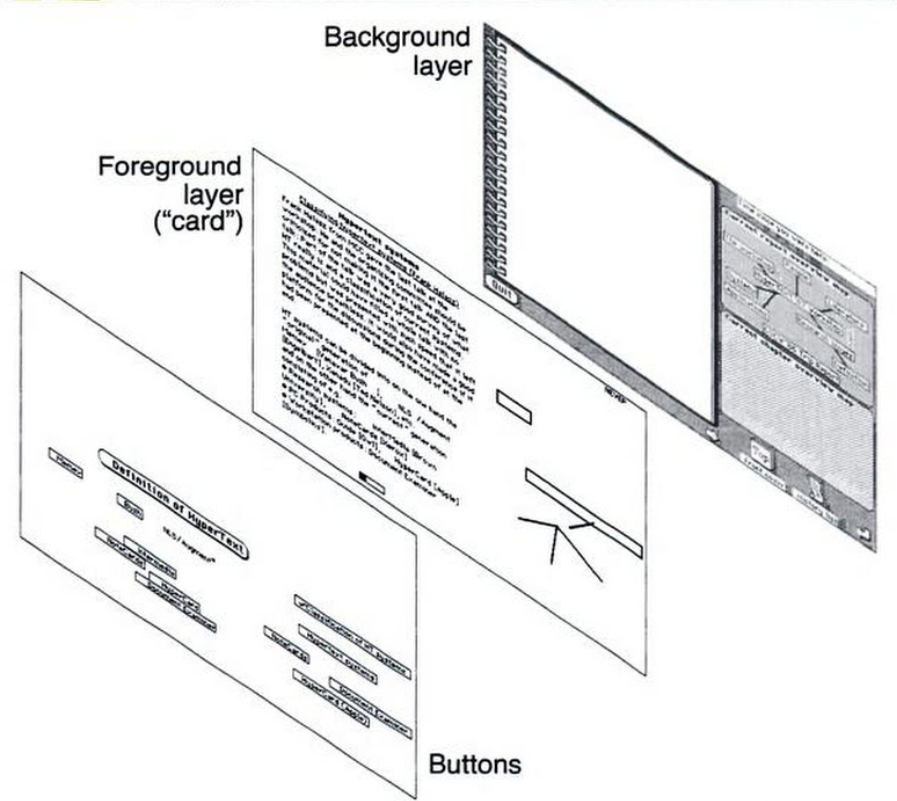
\includegraphics[width=0.9\textwidth]{image/layer}
	\caption{Vereinfachte Ansicht der HyperCard Layer \cite{Nielsen1995}.}
	\label{fig:layer}
\end{figure}

Um einen Link zu erstellen verwendete der Nutzer die Programmiersprache HyperTalk. Ein Beispiel hierfür ist auf der Abbildung \ref{fig:hypercardLink} zusehen. In diesem Beispiel wurde der Hintergrund \glqq Six Monthly\grqq{ }gewählt, beim Klicken auf eine Woche bestimmt das HyperTalk Skript die gewählte Woche und leitet den Nutzer auf die entsprechende Wochenkarte weiter. Es könnten aber auch weitere Berechnungen und Bedingungen die Verlinkung beeinflussen \cite{Goodman1988}, so konnten beliebig komplexe Hypertext entstehen. Ein solcher Link war allerdings immer nur unidirektional, ein Skript auf der Zielkarte konnte aber eine Link zurück anbieten.

\begin{figure}[H]
	\centering
	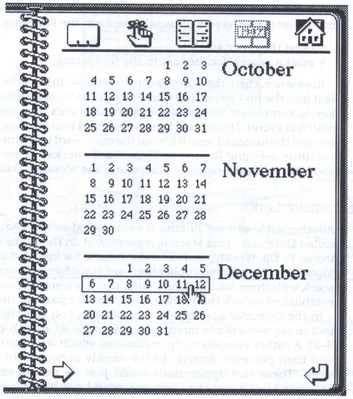
\includegraphics[width=0.9\textwidth]{image/hypercardLink}
	\caption{Ein Beispiel für einen Monat, dargestellt als Card in HyperCard. Beim Klick auf eine Woche wird die entsprechende Card im Termin Stack geöffnet \cite{Goodman1988}.}
	\label{fig:hypercardLink}
\end{figure}

HyperCard identifiziert seine Cards mit der Position innerhalb eines Stacks. Das Problem ist hierbei ist ähnlich wie in Abschnit \ref{sec:dangling} beschrieben. Wenn der Nutzer zum Beispiel die Karte auf Position Zwei in einem Stack löscht, rücken alle späteren Karten nach \cite{Goodman1988}. Allerdings bot HyperCard noch eine andere Möglichkeit auf Cards zu referenzieren. Jede Card erhielt bei der Erstellung eine eindeutige Card ID, keine andere Card in dem Stack konnte diese ID haben. Selbst wenn eine Card gelöscht wurde, wurde die ID nicht erneut vergeben. So konnte zumindest nicht auf eine falsche Card verlinkt werden \cite{Goodman1988}, das Problem einer Dangling Edge konnte trotzdem auftauchen (siehe Abschnitt \ref{sec:dangling}).

\end{section}

\begin{section}{Ist das noch Hypertext?}
\label{sec:nochHypertext}

Die Literatur erwähnt HyperCard oftmals als Hypertext-System \cite{Nielsen1995}, \cite{Dam1988}, \cite{Smith1988}, an dieser Stelle könnte man sich aber folgende Frage stellen: Ist ein System zum Entwickeln grafischer Oberflächen überhaupt noch ein Hypertext-System oder eher schon Programmiersprache? 
Zunächst einmal, was unterscheidet HyperCard von anderen Systemen und Konzepten? Jakob Nielsen schrieb in The learnability of HyperCard as an object-oriented programming system über das System als Programmiersprache, Nutzer mit Programmiererfahrung hätten es leicht die Benutzung von HyperTalk zu verstehen \cite{Nielsen1991}. Aber auch in anderen Systemen, wie das HES, müsse der Nutzer zunächst eine Syntax beherrschen um Text zu verfassen und Links zu erstellen \cite{Dam1969}.

\begin{quote}
\glqq I remember this particular demo we did at Time/Life when our audience said, “That’s great, but it will take us at least 10 years before people will be willing to sit down behind tubes and do anything on-line.”\grqq{ }\cite{Dam1988}
\end{quote}

Auch das Konzept des Main Trails aus der Memex, kann man im wesentlichen mit den Stacks von HyperCard vergleichen. Auch unsere Definitionen aus Kapitel \ref{ch:Was ist Hypertext?} treffen auf HyperCard zu zum Beispiel schrieben John Smith und Stephen Weiss in dem Artikel Hypertext \glqq [...] Hypertext is an approach to information management in which data is stored in a network of nodes connected by links. Nodes can contain text, graphics, audio, video, as well as source code or other forms of data.\grqq{ }\cite{Smith1988} und genau diese Eigenschaften treffen auf HyperCard zu. Informationen sind auf den Cards, die durch Links untereinander verbunden sind.

\begin{quote}
\glqq One of the main design goals of HyperCard was to make it simple and easy to learn.\grqq \cite{Nielsen1991}
\end{quote}

Ein Hypertext-System hat neben der nötigen Benutzerfreundlichkeit für eine hohe Akzeptanz, hat ein solches System aber auch mit andern Problemen zu kämpfen. Da ein Hypertext wie ein wie ein Graph zu betrachten ist und dieser sich bei einigen Anwendungen während der Lebenszeit verändert, können Links ihr Ziel verlieren oder ein Link auf ein falsches Ziel zeigen (Siehe Abschnitt \ref{sec:dangling}). Janet Walker schrieb 1987 in Document Examiner: Delivery Interface for Hypertext Documents: \glqq In most cases so far, the people building the delivery interface are also the people creating the underlying information structure that it is delivering.\grqq{Walker1987}. Ob diese wertende Aussage nun wirklich zutrifft oder nicht soll an dieser Stelle nicht beurteilt werden. Allerdings würde bei einer Vermeidung der dangling Edges bei der Erstellung und vor der Auslieferung, der letztendliche Nutzer dieses Problem niemals zu spüren bekommen.

Vannevar Bush schrieb vom menschlichen Verstand: \glqq The human mind does not work that way. It operarcs by association.\grqq{ }\cite{Bush1945} \cite{Life1945}. Doch das Lost in Hyperspace Problem aus Abschnitt \ref{sec:lostInHyperspace} zeigt, dass Hypertext-Systeme rein nach seinem Konzept nicht unbedingt die optimale Lösung für den menschlichen Verstand sind. Zum Beispiel Hypertext-System wie Document Examiner und HyperCard helfen dem Nutzer mit Metaphern wie einem Buch oder einem Karteikartenstapel, sowie mit Funktionen wie dem Candidates Pane und einer Textsuche.

\end{section}

\chapter{Systeme}
\label{ch:Systeme}


\begin{section}{Document Examiner}
\label{sec:DocumentExaminer}

1985
Symbolics Inc.
Symbolics Handbücher
Concordia als Editor
An die Recherche in Handbüchern angepasst
Content area, Kandidaten, Bookmarks, Command region
Ein Klick auf einen Link fügt zu Kandidaten hinzu
Inspiriert von NLS, Xanadu und HES
Records enthalten Titel und Beschreibung
Record hat ID
Sequenzen von Records

\end{section}


\chapter{Nutzung}
\label{ch:Nutzung}

\begin{section}{Nutzungsgeschichten}
\label{sec:Nutzungsgeschichten}

Lorem ipsum dolor sit amet, consetetur sadipscing elitr, sed diam nonumy eirmod tempor invidunt ut labore et dolore magna aliquyam erat, sed diam voluptua. At vero eos et accusam et justo duo dolores et ea rebum. Stet clita kasd gubergren, no sea takimata sanctus est Lorem ipsum dolor sit amet. Lorem ipsum dolor sit amet, consetetur sadipscing elitr, sed diam nonumy eirmod tempor invidunt ut labore et dolore magna aliquyam erat, sed diam voluptua. At vero eos et accusam et justo duo dolores et ea rebum. Stet clita kasd gubergren, no sea takimata sanctus est Lorem ipsum dolor sit amet.

\end{section}

\begin{section}{Funktionen}
\label{sec:Funktionen}

Lorem ipsum dolor sit amet, consetetur sadipscing elitr, sed diam nonumy eirmod tempor invidunt ut labore et dolore magna aliquyam erat, sed diam voluptua. At vero eos et accusam et justo duo dolores et ea rebum. Stet clita kasd gubergren, no sea takimata sanctus est Lorem ipsum dolor sit amet. Lorem ipsum dolor sit amet, consetetur sadipscing elitr, sed diam nonumy eirmod tempor invidunt ut labore et dolore magna aliquyam erat, sed diam voluptua. At vero eos et accusam et justo duo dolores et ea rebum. Stet clita kasd gubergren, no sea takimata sanctus est Lorem ipsum dolor sit amet.

\end{section}

\begin{section}{Problem: Lost in Hyperspace}
\label{sec:LostInHyperspace}

Lorem ipsum dolor sit amet, consetetur sadipscing elitr, sed diam nonumy eirmod tempor invidunt ut labore et dolore magna aliquyam erat, sed diam voluptua. At vero eos et accusam et justo duo dolores et ea rebum. Stet clita kasd gubergren, no sea takimata sanctus est Lorem ipsum dolor sit amet. Lorem ipsum dolor sit amet, consetetur sadipscing elitr, sed diam nonumy eirmod tempor invidunt ut labore et dolore magna aliquyam erat, sed diam voluptua. At vero eos et accusam et justo duo dolores et ea rebum. Stet clita kasd gubergren, no sea takimata sanctus est Lorem ipsum dolor sit amet.

\end{section}


\chapter{Technik}
\label{ch:Technik}


\begin{section}{Technische Vorraussetzungen}
\label{sec:TechnischeVorraussetzungen}

Lorem ipsum dolor sit amet, consetetur sadipscing elitr, sed diam nonumy eirmod tempor invidunt ut labore et dolore magna aliquyam erat, sed diam voluptua. At vero eos et accusam et justo duo dolores et ea rebum. Stet clita kasd gubergren, no sea takimata sanctus est Lorem ipsum dolor sit amet. Lorem ipsum dolor sit amet, consetetur sadipscing elitr, sed diam nonumy eirmod tempor invidunt ut labore et dolore magna aliquyam erat, sed diam voluptua. At vero eos et accusam et justo duo dolores et ea rebum. Stet clita kasd gubergren, no sea takimata sanctus est Lorem ipsum dolor sit amet.

\end{section}

\begin{section}{Private und öffentliche Links}
\label{sec:links}

Lorem ipsum dolor sit amet, consetetur sadipscing elitr, sed diam nonumy eirmod tempor invidunt ut labore et dolore magna aliquyam erat, sed diam voluptua. At vero eos et accusam et justo duo dolores et ea rebum. Stet clita kasd gubergren, no sea takimata sanctus est Lorem ipsum dolor sit amet. Lorem ipsum dolor sit amet, consetetur sadipscing elitr, sed diam nonumy eirmod tempor invidunt ut labore et dolore magna aliquyam erat, sed diam voluptua. At vero eos et accusam et justo duo dolores et ea rebum. Stet clita kasd gubergren, no sea takimata sanctus est Lorem ipsum dolor sit amet.

\end{section}

\begin{section}{Problem: Dangling edges}
\label{sec:dangling}

Lorem ipsum dolor sit amet, consetetur sadipscing elitr, sed diam nonumy eirmod tempor invidunt ut labore et dolore magna aliquyam erat, sed diam voluptua. At vero eos et accusam et justo duo dolores et ea rebum. Stet clita kasd gubergren, no sea takimata sanctus est Lorem ipsum dolor sit amet. Lorem ipsum dolor sit amet, consetetur sadipscing elitr, sed diam nonumy eirmod tempor invidunt ut labore et dolore magna aliquyam erat, sed diam voluptua. At vero eos et accusam et justo duo dolores et ea rebum. Stet clita kasd gubergren, no sea takimata sanctus est Lorem ipsum dolor sit amet.

\end{section}

\begin{section}{Technische Entwicklung lassen Nutzungsformen entstehen?}
\label{sec:entwicklung}

Lorem ipsum dolor sit amet, consetetur sadipscing elitr, sed diam nonumy eirmod tempor invidunt ut labore et dolore magna aliquyam erat, sed diam voluptua. At vero eos et accusam et justo duo dolores et ea rebum. Stet clita kasd gubergren, no sea takimata sanctus est Lorem ipsum dolor sit amet. Lorem ipsum dolor sit amet, consetetur sadipscing elitr, sed diam nonumy eirmod tempor invidunt ut labore et dolore magna aliquyam erat, sed diam voluptua. At vero eos et accusam et justo duo dolores et ea rebum. Stet clita kasd gubergren, no sea takimata sanctus est Lorem ipsum dolor sit amet.

\end{section}




\chapter{Zusammenfassung}
\label{ch:Zusammenfassung}


\nocite{BPR}
\pagenumbering{Roman}
\bibliography{bib/Literatur}
%\lstlistoflistings
%\listoffigures

\end{document}